\documentclass[11pt]{article}
\usepackage[a4paper, margin=1in]{geometry}
\usepackage[utf8]{inputenc}
\usepackage{amsmath,titlesec}
\usepackage{graphicx}
\usepackage{wrapfig}
\titleformat*{\subsection}{\normalfont\large\itshape\titlerule}

\title{Lab 4 - Tutorial Writing}
\author{Ratun Rahman, 170042011}
\date{August 2021}

\begin{document}

\begin{titlepage}
\maketitle
\end{titlepage}

\begin{center} \Huge{\textbf{Gradient Descent}}
\end{center}
\section*{1 Introduction}
\subsection*{}
\textbf{Gradient descent} is an optimization algorithm for finding a local minimum of a differentiable function. Gradient descent is simply used in machine learning to find the values of a function's parameters (coefficients) that minimize a cost function as far as possible. You start by defining the initial parameter's values and from there gradient descent uses calculus to iteratively adjust the values so they minimize the given cost-function. To understand this concept full, it's important to know about gradients. \\
\begin{figure}[htp]
    \centering
    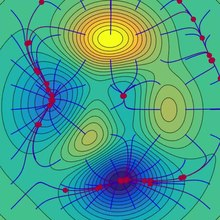
\includegraphics[width=5cm]{photo/1.jpg}
    \caption{Gradient Descent in 2D}
    \label{fig:ss1}
\end{figure}
\textbf{Gradient descent} is generally attributed to Cauchy, who first suggested it in 1847. Hadamard independently proposed a similar method in 1907. Its convergence properties for non-linear optimization problems were first studied by \textbf{Haskell Curry} in 1944, with the method becoming increasingly well-studied and used in the following decades, also often called steepest descent. 

\section*{2 Problem Formulation}
\subsection*{}
\begin{wrapfigure}{r}{0.25\textwidth}
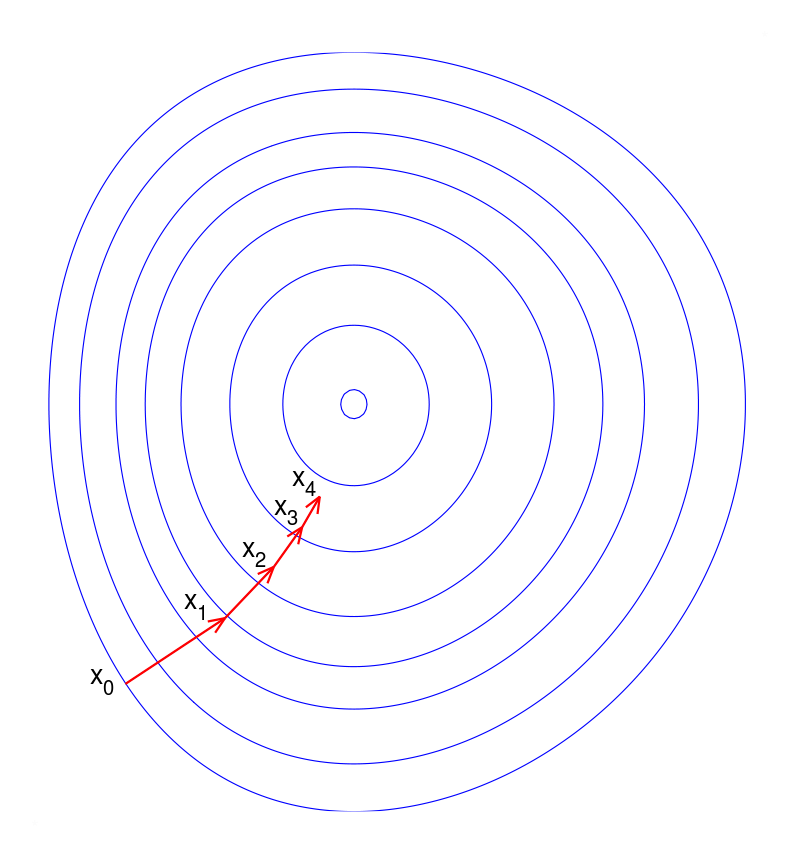
\includegraphics[width=0.9\linewidth]{photo/2.png} 
\caption{Illustration of gradient descent on a series of level sets}
\label{fig:wrapfig}
\end{wrapfigure}
Gradient descent is based on the observation that if the multi-variable function F(x) is defined and differentiable in a neighborhood of a point a, then F(x) a in the direction of the negative gradient of F at a, -\(\nabla\) F(a). It follows that, if

    \[a_{n + 1}=\mathbf {a} _{n}-\gamma \nabla F(\mathbf {a} _{n})\]

for a \(\gamma \in R_+\) small enough, then \(F(a_{n})\geq F(a_{n+1})\). In other words, the term \( \gamma \nabla F(a)\) is subtracted from a because we want to move against the gradient, toward the local minimum. With this observation in mind, one starts with a guess \( x_0\) for a local minimum of F, and considers the sequence \(  x_0, x_1, x_2,\dots\) such that

    \[ \mathbf {x} _{n+1}=\mathbf {x} _{n}-\gamma _{n}\nabla F(\mathbf {x} _{n}),\ n\geq 0\]
We have a monotonic sequence,

    \[F(\mathbf {x} _{0})\geq F(\mathbf {x} _{1})\geq F(\mathbf {x} _{2})\geq \cdots\]
    
So, hopefully, the sequence \(\mathbf {x} _{n}\) converges to the desired local minimum. Note that the value of the step size \(\gamma\) is allowed to change at every iteration. With certain assumptions on the function F (for example, F convex and \(\nabla F\) Lipschitz) and particular choices of \(\gamma\) (e.g., chosen either via a line search that satisfies the Wolfe conditions, or the Barzilai–Borwein method shown as following),

    \[\gamma _{n}={\frac {\left|\left(\mathbf {x} _{n}-\mathbf {x} _{n-1}\right)^{T}\left[\nabla F(\mathbf {x} _{n})-\nabla F(\mathbf {x} _{n-1})\right]\right|}{\left\|\nabla F(\mathbf {x} _{n})-\nabla F(\mathbf {x} _{n-1})\right\|^{2}}}\]

convergence to a local minimum can be guaranteed. When the function F is convex, all local minima are also global minima, so in this case gradient descent can converge to the global solution.

This process is illustrated in the adjacent picture. Here, F is assumed to be defined on the plane, and that its graph has a bowl shape. The blue curves are the contour lines, that is, the regions on which the value of F is constant. A red arrow originating at a point shows the direction of the negative gradient at that point. Note that the (negative) gradient at a point is orthogonal to the contour line going through that point. We see that gradient descent leads us to the bottom of the bowl, that is, to the point where the value of the function F is minimal. 
\section*{3 General Solution}
\subsection*{}
Since using a step size \(\gamma\) that is too small would slow convergence, and a \(\gamma\) too large would lead to divergence, finding a good setting of \(\gamma\) is an important practical problem. Philip Wolfe also advocated for using "clever choices of the [descent] direction" in practice. Whilst using a direction that deviates from the steepest descent direction may seem counter-intuitive, the idea is that the smaller slope may be compensated for by being sustained over a much longer distance.

To reason about this mathematically, let's use a direction \(\mathbf {p} _{n}\) and step size \(\gamma _{n}\) and consider the more general update:

    \[ \mathbf {a} _{n+1}=\mathbf {a} _{n}-\gamma _{n}\,\mathbf {p} _{n}\].

Finding good settings of \( \mathbf {p} _{n}\) and \( \gamma _{n}\) requires a little thought. First of all, we would like the update direction to point downhill. Mathematically, letting \( \theta _{n}\) denote the angle between \( \nabla F(\mathbf {a_{n}} )\) and \( \mathbf {p} _{n}\), this requires that \( \cos \theta _{n}>0.\) To say more, we need more information about the objective function that we are optimising. Under the fairly weak assumption that F is continuously differentiable, we may prove that:
\begin{equation}
    F(\mathbf {a} _{n+1})\leq F(\mathbf {a} _{n})-\gamma _{n}\|\nabla F(\mathbf {a} _{n})\|_{2}\|\mathbf {p} _{n}\|_{2}\left[\cos \theta _{n}-\max _{t\in [0,1]}{\frac {\|\nabla F(\mathbf {a} _{n}-t\gamma _{n}\mathbf {p} _{n})-\nabla F(\mathbf {a} _{n})\|_{2}}{\|\nabla F(\mathbf {a} _{n})\|_{2}}}\right]
\end{equation}

This inequality implies that the amount by which we can be sure the function F is decreased depends on a trade off between the two terms in square brackets. The first term in square brackets measures the angle between the descent direction and the negative gradient. The second term measures how quickly the gradient changes along the descent direction.
\begin{figure}
    \centering
    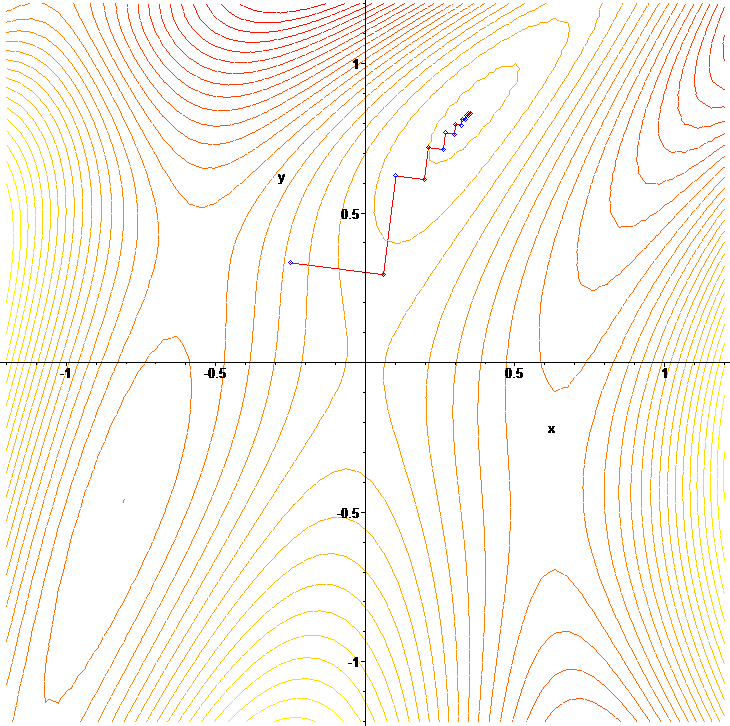
\includegraphics[width=9cm]{photo/4.png}
    \caption{The gradient descent algorithm in action (contour)}
    \label{fig:ss2}
\end{figure}
In principle inequality (1) could be optimized over \(\mathbf {p} _{n}\) and \(\gamma _{n}\) to choose an optimal step size and direction. The problem is that evaluating the second term in square brackets requires evaluating \(\nabla F(\mathbf {a} _{n}-t\gamma _{n}\mathbf {p} _{n})\), and extra gradient evaluations are generally expensive and undesirable. Some ways around this problem are:\\

    1. Forgo the benefits of a clever descent direction by setting \( \mathbf {p} _{n}=\nabla F(\mathbf {a_n} )\), and use line search to find a suitable step-size \(\gamma _n\), such as one that satisfies the Wolfe conditions.
    
    2. Assuming that F is twice-differentiable, use its Hessian \(\nabla ^{2}F\) to estimate \[ \|\nabla F(\mathbf {a} _{n}-t\gamma _{n}\mathbf {p} _{n})-\nabla F(\mathbf{a}_{n})\|_{2}\approx \|t\gamma _{n}\nabla ^{2}F(\mathbf {a} _{n})\mathbf {p} _{n}\|.\] Then choose \( \mathbf {p} _{n}\) and \(\gamma _{n}\) by optimising inequality (1).
    
    3. Assuming that \(\nabla F\) is Lipschitz, use its Lipschitz constant L to bound \( \|\nabla F(\mathbf {a} _{n}-t\gamma _{n}\mathbf {p} _{n})-\nabla F(\mathbf {a} _{n})\|_{2}\leq Lt\gamma _{n}\|\mathbf {p} _{n}\|.\) Then choose \(\mathbf {p} _{n}\) and \( \gamma _{n}\) by optimising inequality (1).
    
    4. Build a custom model of \[ \max _{t\in [0,1]}{\frac {\|\nabla F(\mathbf {a} _{n}-t\gamma _{n}\mathbf {p} _{n})-\nabla F(\mathbf {a} _{n})\|_{2}}{\|\nabla F(\mathbf {a} _{n})\|_{2}}}\] for F. Then choose \(\mathbf {p} _{n}\) and \(\gamma _{n}\) by optimising inequality (1).
    
    5. Under stronger assumptions on the function F such as convexity, more advanced techniques may be possible.

Usually by following one of the recipes above, convergence to a local minimum can be guaranteed. When the function F is convex, all local minima are also global minima, so in this case gradient descent can converge to the global solution. 
\section*{4 Example}
\subsection*{}
Consider the nonlinear system of equations

    \[{\begin{cases}3x_{1}-\cos(x_{2}x_{3})-{\tfrac {3}{2}}=0\\4x_{1}^{2}-625x_{2}^{2}+2x_{2}-1=0\\\exp(-x_{1}x_{2})+20x_{3}+{\tfrac {10\pi -3}{3}}=0\end{cases}}\]

Let us introduce the associated function

    \[ G(\mathbf {x} )={\begin{bmatrix}3x_{1}-\cos(x_{2}x_{3})-{\tfrac {3}{2}}\\4x_{1}^{2}-625x_{2}^{2}+2x_{2}-1\\\exp(-x_{1}x_{2})+20x_{3}+{\tfrac {10\pi -3}{3}}\\\end{bmatrix}}\]

where

    \[\mathbf {x} ={\begin{bmatrix}x_{1}\\x_{2}\\x_{3}\\\end{bmatrix}}\]

One might now define the objective function

    \[ F(\mathbf {x} )={\frac {1}{2}}G^{\mathrm {T} }(\mathbf {x} )G(\mathbf {x} )\]
    \[={\frac{1}{2}}\left[\left(3x_{1}-\cos(x_{2}x_{3})-{\frac{3}{2}}\right)^{2}+\left(4x_{1}^{2}-625x_{2}^{2}+2x_{2}-1\right)^{2}+\left(\exp(-x_{1}x_{2})+20x_{3}+{\frac{10\pi-3}{3}}\right)^{2}\right],\]

which we will attempt to minimize. As an initial guess, let us use

    \[ \mathbf {x} ^{(0)}=\mathbf {0} ={\begin{bmatrix}0\\0\\0\\\end{bmatrix}}\]

We know that

    \[ \mathbf {x} ^{(1)}=\mathbf {0} -\gamma _{0}\nabla F(\mathbf {0} )=\mathbf {0} -\gamma _{0}J_{G}(\mathbf {0} )^{\mathrm {T} }G(\mathbf {0} )\]

where the Jacobian matrix \( J_{G}\) is given by

    \[ J_{G}(\mathbf {x} )={\begin{bmatrix}3&\sin(x_{2}x_{3})x_{3}&\sin(x_{2}x_{3})x_{2}\\8x_{1}&-1250x_{2}+2&0\\-x_{2}\exp {(-x_{1}x_{2})}&-x_{1}\exp(-x_{1}x_{2})&20\\\end{bmatrix}}.\]

We calculate:

    \[ J_{G}(\mathbf {0} )={\begin{bmatrix}3&0&0\\0&2&0\\0&0&20\end{bmatrix}},\qquad G(\mathbf {0} )={\begin{bmatrix}-2.5\\-1\\10.472\end{bmatrix}}\]

Thus

    \[ \mathbf {x} ^{(1)}=\mathbf {0} -\gamma _{0}{\begin{bmatrix}-7.5\\-2\\209.44\end{bmatrix}}\]

and

    \[ F(\mathbf {0} )=0.5\left((-2.5)^{2}+(-1)^{2}+(10.472)^{2}\right)=58.456\]
Now, a suitable \(\gamma _{0}\) must be found such that

    \[ F\left(\mathbf {x} ^{(1)}\right)\leq F\left(\mathbf {x} ^{(0)}\right)=F(\mathbf {0} )\]

This can be done with any of a variety of line search algorithms. One might also simply guess \( \gamma _{0}=0.001,\) which gives

    \[ \mathbf {x} ^{(1)}={\begin{bmatrix}0.0075\\0.002\\-0.20944\\\end{bmatrix}}\]

\begin{wrapfigure}{r}{0.25\textwidth}
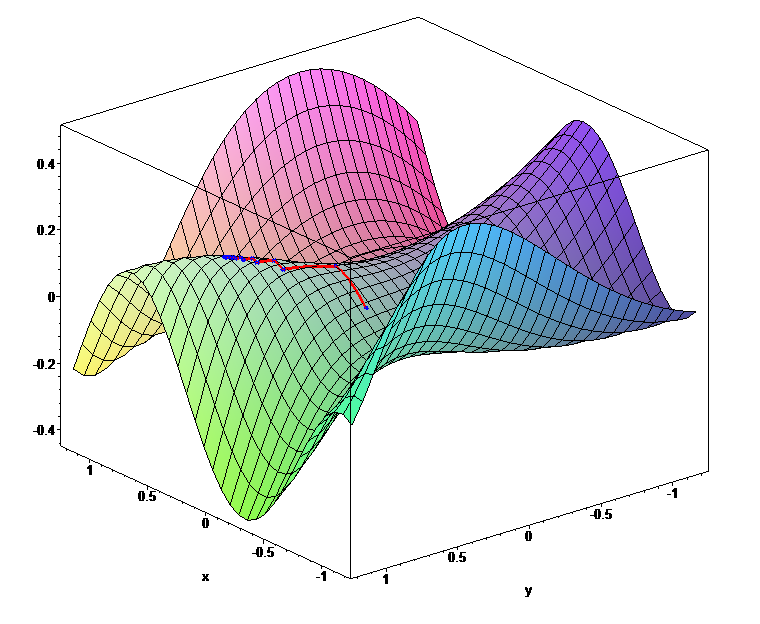
\includegraphics[width=0.9\linewidth]{photo/3.png} 
\caption{The gradient descent algorithm in action}
\label{fig:wrapfig2}
\end{wrapfigure}
Evaluating the objective function at this value, yields

    \[ F\left(\mathbf {x} ^{(1)}\right)=0.5\left((-2.48)^{2}+(-1.00)^{2}+(6.28)^{2}\right)=23.306\]

The decrease from F(0) = 58.456 to the next step's value of

    \[ F\left(\mathbf {x} ^{(1)}\right)=23.306\]

is a sizable decrease in the objective function. Further steps would reduce its value further, until an approximate solution to the system was found. 
\section*{5 Complexity Analysis}
\subsection*{}
according to the Machine Learning course by Stanford University, the complexity of gradient descent is \(O(kn^2)\), where

k= Number of iteration

n= Number of variables\\
When n is very large, it is recommended to use Gradient Descent algorithm.
\end{document}
